\documentclass[../main.tex]{subfiles}
\graphicspath{{\subfix{../images/}}}
\begin{document}
\section*{Term 2 Week 5}
\begin{enumerate}
    \item 
    Find the \textbf{exact} area of the shaded square inside the regular hexagon with side lengths of 1.\\
    \begin{figure}[h]
        \centering
        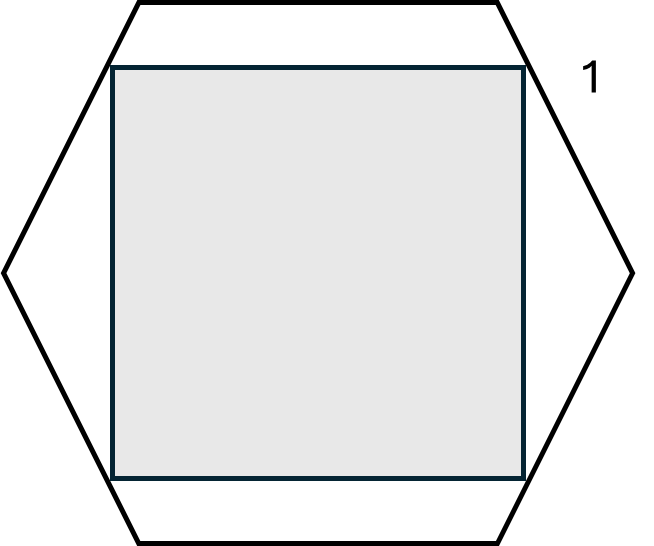
\includegraphics{images/t2w5q1.png}
    \end{figure}

    \item 
    Find the derivative of \(y=x^{x^{x^{x^{.^{.^{.}}}}}}\)\\

    \item 
    We define \(a=1+\frac{x}{y}\) and \(b=1+\frac{y}{x}\), where \textit{a} and \textit{b} are positive real numbers.\\

    If \(a^2+b^2=15\), find the value of \(a^3+b^3\).\\

    \item 
    Find the sum of all real solutions to the equation \(x^2+\cos{(x)}=2024 \)
    
    \end{enumerate}

\end{document}